\documentclass{article} % For LaTeX2e
\usepackage{nips14submit_e,times}
\usepackage{hyperref}
\usepackage{url}
\usepackage{amsmath}
\usepackage{graphicx}
\usepackage{subcaption}
%\documentstyle[nips14submit_09,times,art10]{article} % For LaTeX 2.09

\title{Autoencoded $k$-means: Using jointly trained autoencoders for robust clustering}

\author{
Colin Samplawski \\
College of Information and Computer Sciences\\
University of Massachusetts Amherst\\
\texttt{csamplawski@cs.umass.edu} \\
}

\newcommand{\fix}{\marginpar{FIX}}
\newcommand{\new}{\marginpar{NEW}}

\nipsfinalcopy

\begin{document}

\maketitle

\begin{abstract}
The classical methods for $k$-means clustering can perform poorly in high dimensional feature spaces or in the presence of noise. This motivates the addition of an autoencoder architecture to simultaneously reduce the dimensionality of the data and remove noise. In this work, I provide a model which jointly trains a denoising autoencoder and optimizes the $k$-means objective. I see that my model is capable of producing higher quality clusterings than the standard algorithm.
\end{abstract}

\section{Introduction}
The workhorse method for data clustering is $k$-means. Given a dataset of $N$ points $\{x_1,x_2,\dots, x_N\}$, the algorithm finds $k$ cluster centers $C=\{c_1,c_2,\dots,c_k \}$ which minimize the sum of the distances between each data point and the cluster center that it is closest to. This can be expressed as the following objective:
\begin{equation}
\mathcal{L} = \sum_{i=1}^N \min_{c_j \in C} ||x_i - c_j||^2
\end{equation}
Since $k$-means uses squared Euclidean distance, all the features of the data contribute equally to the distance calculation. This can be problematic in high dimensional features spaces since some features may be uninformative. Furthermore, it has been shown that $k$-means performs poorly in the presence of noise \cite{noisecluster}. This motivates the addition of an autoencoder.

An autoencoder is a neural network which learns to reproduce its input. In the most basic setting, it consists of a single hidden layer followed by a linear output layer that is equal in size to the input. If we set the hidden layer size to be less than the input size, we can train the autoencoder to produce representations of the data in a smaller dimensional space. This implicitly performs feature selection on the data. The computations of the autoencoder are as follows:
\begin{equation}
\begin{aligned}
h &= f(xW_1 + b_1)\\
x' &= hW_2 + b_2
\end{aligned}
\end{equation}
where $f$ is a nonlinearity, $W_1,W_2$ are the weights of the network, and $b_1,b_2$ are the biases. We call $x'$ the reconstruction of the input $x$ and $h$ the hidden state. We train to minimize the reconstruction error, given by:
\begin{equation}
\sum_{i=1}^N ||x_i - x_i'||^2
\end{equation}
Autoencoders have been shown to be an effective way to reduce dimensionality in an unsupervised way \cite{noiseae}. Furthermore, they can be extended to also denoise data. A denoising autoencoder has nearly the same architecture as above, only a noisy version of the input is given at training time. The reconstruction error is then calculated using the clean version of the input. Denoising autoencoders have been shown to be an effective method of denoising data \cite{noiseae}. In this work I provide an architecture which jointly learns a denoising autoencoder and optimizes the $k$-means objective.

The rest of this paper is structured as follows: Section 2 discusses relevant previous work. Section 3 provides a short overview of cluster evaluation metrics. In Section 4 I describe the model architecture. Section 5 discusses experimental design and results.  Section 6 discusses possible future work. Finally, Section 7 concludes.

\section{Related Work}
The traditional method of handling uninformative features is weighted $k$-means \cite{weighted}. By assigning a weight to each feature, uninformative features won't play as large of a role in the cluster distance calculation, which can lead to improved performance. Unfortunately, this is not usually feasible since it requires domain knowledge at the feature level, which often doesn't exist. Furthermore, it does little in the face of noisy data.

The use of autoencoders to improve clustering performance has a reasonable body of prior work. Most relevant to this work is the work done by Xie et al. \cite{deepcluster}. They jointly trained a deep autoencoder and optimized a clustering objective to improve clustering of textual and image data. However, unlike my work, they used gradient descent to optimize KL-divergence for clustering.  

Tian et al. used autoencoders to improve the performance of graph clustering \cite{graph}. Coates et al.  showed that autoencoders can be an effective method of extracting features from image data \cite{coates}. They also demonstrated that $k$-means could successively cluster images, however, the two were not used together. Finally, Dilokthanakul et al. used variational autoencoders to improve clustering using Gaussian mixture models \cite{gmm}.

\section{Cluster Evaluation}
Evaluating clusterings is generally a more difficult task than the case of classification. Fortunately, the datasets I am using have ground truth labels, so we can use metrics which take advantage of that information. I used three commonly used cluster performance metrics to evaluate the clusterings produced by my model. These three were chosen because they share many proprieties. Namely, they all have range [0,1], and they output 0 in the case of random assignments and 1 in the case of perfect clustering. Also, all three are insensitive to the number of clusters used, unlike other metrics, such as cluster purity. All three metrics were calculated using implementations found in scikit-learn's metric package.\footnote{\texttt{http://scikit-learn.org/stable/modules/model\_evaluation.html}} I now provide a brief summary of each metric. Let $D$ be a dataset of $N$ points, $C$ be clusters of points from $D$, and $L$ be the ground truth labels.

\subsection{V-Measure}
The V-measure (validity measure) is an entropy based clustering metric which measures a clusterings trade-off between homogeneity ($h$) and completeness ($c$). A cluster is homogeneous if it contains points that all are of the same class. A clustering is complete if points from the same class are assigned to the same cluster. They are defined as follows:
\begin{equation}
h =
\begin{cases}
1 & \text{if } H(L, C) = 0 \\
1 - \frac{H(L|C)}{H(L)} & \text{else}
\end{cases}
\qquad 
c =
\begin{cases}
1 & \text{if } H(C, L) = 0 \\
1 - \frac{H(C|L)}{H(C)} & \text{else}
\end{cases}
\end{equation}  
where $H$  is information entropy. Note that these components often are opposing, increasing one usually decreases the other.  V-measure is then the harmonic mean of homogeneity and completeness:
\begin{equation}
\frac{2 \cdot c \cdot h}{c+h}
\end{equation}
In this way, it is somewhat analogous to the F1 measure commonly used in information extraction. A full analysis of V-Measure can be found in \cite{vmeasure}.

\subsection{Normalized Mutual Information}
Normalized Mutual information (NMI) is an information theoretic metric which is defined as follows:  
\begin{equation}
\frac{I(C;L)}{H(C)+H(L)}
\end{equation}
where $I(C;L)$ is the mutual information between $C$ and $L$, and $H$ is  again entropy. An in depth discussion of this and other information theoretic metrics can be found in \cite{info}.

\subsection{Rand Score}
The Rand score, named after William M. Rand, measures the similarity of two partitions of a dataset. The Rand score is defined as:
\begin{equation}
\frac{a+b}{\binom{N}{2}}
\end{equation}
where $a$ is the number of pairs of points that are in the same subset in $C$ and in the same subset in $L$, and $b$ is the number of pairs of points  that are in different subsets in $C$ and in different subsets in $L$. Note that $\binom{N}{2}$ is the total number of pairs of points in $D$. A full analysis of this metric can be found in \cite{rand}.




\section{Model}
\subsection{Gradient $k$-means}
Most implementations of $k$-means work without the use of gradient methods, usually by using Lloyd's algorithm 
\cite{lloyd}. However, a gradient descent version of $k$-means is fairly simple to derive. Following the derivation provided by Bottou and Bengio \cite{convergence}, we frame $k$-means as the following minimization problem:
\begin{equation}
\min \mathcal{L} = \min \sum_{i=1}^N \frac{1}{2} ||x_i - c_{x_i}||^2
\end{equation}
where $c_{x_i}$ is the closest cluster center to data point $x_i$. This then gives the following gradient: 
\begin{equation}
\frac{\partial \mathcal{L}}{\partial c_j} = \sum_{i=1}^N 
\begin{cases}
x_i - c_j  &  \text{if } c_j = c_{x_i} \\
0& \text{else} \\
\end{cases}
\end{equation} 
With the gradient in hand, we can use a gradient descent algorithm to perform $k$-means clustering. In fact, Sculley has shown that a mini-batched version of this approach converges faster than any other algorithm when working in a large data regime \cite{Sculley}. We will call this model gradient $k$-means. As a baseline for my model, I implemented mini-batched gradient $k$-means in Tensorflow, which did not exist elsewhere to the best of my knowledge. Table \ref{sklearn} shows that it generates clusterings of higher quality than the algorithm provided by scikit-learn.\footnote{\texttt{http://scikit-learn.org/stable/modules/generated/sklearn.cluster.MiniBatchKMeans.html}}

\begin{table}
	\caption{Comparison of $k$-means implementations. We compare scikit-learn's MiniBatchKMeans method$^2$  and my gradient $k$-means implementation. We see that my implementation results in higher quality clusterings for both datasets (Section 5.1).}
	\label{sklearn}
	\begin{center}
	\begin{tabular}{|c |c c |c c|}
		\multicolumn{1}{c}{} & \multicolumn{2}{c}{MNIST}   &\multicolumn{2}{c}{EMNIST}   \\
		\hline
		Score & scikit-learn & Gradient $k$-means & scikit-learn & Gradient $k$-means\\
		\hline \hline
	    V-Measure & 0.514 & 0.533 & 0.466 & 0.467 \\ 
		NMI & 0.387 & 0.441 & 0.368 & 0.372\\  
		Rand Score & 0.138 & 0.338 & 0.089 & 0.185\\
		\hline
	\end{tabular}
	\end{center}
\end{table}

\subsection{Autoencoded $k$-means}
Since gradient $k$-means produces gradients, we can backpropagate the error signal from the $k$-means objective through a neural architecture. I have a designed a  model which consists of an autoencoder whose hidden state is given as input to gradient $k$-means (Figure \ref{fig:grad_kmeans}). We will refer to this model as autoencoded $k$-means. During training, the error signals from both the autoencoder reconstruction and gradient $k$-means is backpropagated jointly through the hidden state. In this way, we are not only learning a smaller representation for the input, we are biasing that representation to be well suited for clustering. The objective for the entire architecture is: 
\begin{equation}
\frac{1}{N}\sum_{i=1}^N \frac{1}{F} ||x_i-x_i'||^2 + \frac{1}{N}\sum_{i=1}^N \frac{1}{2} ||h_i - c_{h_i}||^2
\end{equation}
where $F$ is the number of features.
\begin{figure}
	\begin{center}
		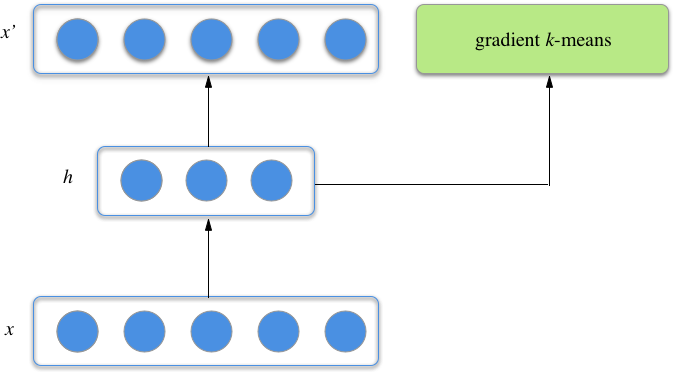
\includegraphics[width=0.6\textwidth]{figs/akm.png}
	\end{center}
	\caption{The autoencoded $k$-means architecture.}
	\label{fig:grad_kmeans}
\end{figure}

\section{Experiments}
\subsection{Datasets}
To test my model I used two image datasets. I chose to use image data because they have a large number of features, even for simple images, and noise can be easily added artificially. In particular, I ran my experiments on the MNIST \cite{mnist} and EMNIST \cite{emnist} datasets (Figure \ref{fig:datasets}). MNIST is a classical dataset in image processing which consists of 60,000 handwritten digits displayed in 28x28 gray-scale images. EMNIST (extended MNIST) is a recent dataset which consists of images in the same format as MNIST, but includes letters A-Z as well as digits. For this work, I only considered the 124,800 images from the dataset which were of a letter. Letters in the dataset can be upper or lowercase, however, there is only 26 classes. That is, images of ``a" and ``A" are considered the same class.

\begin{figure}
	\centering
	\begin{subfigure}[b]{\textwidth}
		
\includegraphics[width=\textwidth]{figs/mnist.png}
	\end{subfigure}
	\begin{subfigure}[b]{\textwidth}
		
\includegraphics[width=\textwidth]{figs/emnist.png}
	\end{subfigure}
	\caption{Sample images. MNIST (upper) consists of handwritten digits 0-9 and EMNIST (lower) consists of handwritten letters a-z and A-Z. Both consist of 28x28 centered gray-scale images.}
	\label{fig:datasets}
\end{figure}

\subsection{Implementation Details}
All my experiments and models were developed using Tensorflow\footnote{\texttt{https://www.tensorflow.org}} (my code is publicly available\footnote{\texttt{https://github.com/colinski/AutoencodedKMeans}}). For both datasets a batch size of 100 was used. Optimization was performed via the Adam optimizer \cite{adam} using the default parameters of the Tensorflow implementation\footnote{\texttt{https://www.tensorflow.org/api\_docs/python/tf/train/AdamOptimizer}}. The number of clusters used was determined to be 10 times the number of classes, so 100 for MNIST and 260 for EMNIST. The autoencoder used a tanh nonlinearity. The matrix of cluster centers was initialized as the pseudo-identity matrix, and the weights and biases of the autoencoder was initialized using the Xavier initialization method \cite{xavier}. Training took place on a GPU.

\subsection{Effect of Representation Dimension}
We first experiment by changing the size of the representation produced by the autoencoder. For a range of values (2 at the lowest, 400 at the highest), I trained autoencoded $k$-means to learn a representation of that size and simultaneously cluster the data in that smaller dimensional feature space. We hope that the autoenocder will select the most informative features, resulting in better clustering. The results of these experiments can be found in Figure \ref{fig:dims}

We see a significant decrease in performance on both datasets for small dimensional values (2 and 64) when compared to $k$-means. This isn't surprising since it seems unlikely that a 784 feature space could be reasonably represented in 2. However, once a reasonable dimension size is reached, we see an increase in performance  on both datasets. MNIST especially shows sizable gains over $k$-means for a dimension of size 256. Interestingly, as the dimension size increases past 256, we see a drop in performance on the MNIST data. This suggests that the autoencoder may be preserving unimportant features in its representation, leading to worse clustering performance.

From these experiments we see that EMNIST is significantly harder dataset to cluster. This isn't surprising given the increased complexity of the data. Autoencoded $k$-means is able to gain a small performance gain over $k$-means, however it scores consistently worse on the V-Measure metric, across all choices of dimension size. This is due to the fact that the completeness component of the V-Measure on the EMNIST data was consistently low. This means that points from the same class aren't being assigned to the same cluster. This may be due to the fact that EMNIST treats upper and lowercase letters as the same class. It seems likely that autoencoded $k$-means is learning to place ``a" in a different cluster than ``A", resulting in lower completeness.

\begin{figure}
	\centering
	\begin{minipage}[b]{0.45\textwidth}
		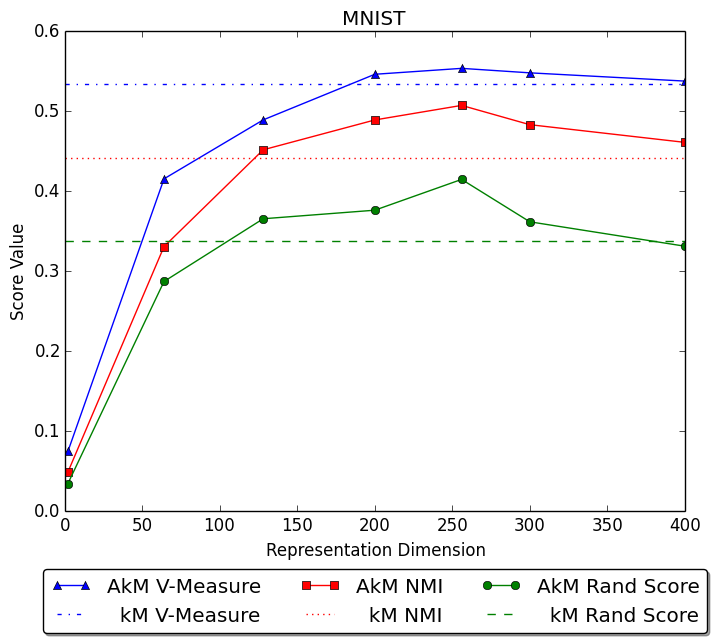
\includegraphics[width=\textwidth]{figs/mnist_graph.png}
	\end{minipage}
	\hfill
	\begin{minipage}[b]{0.45\textwidth}
		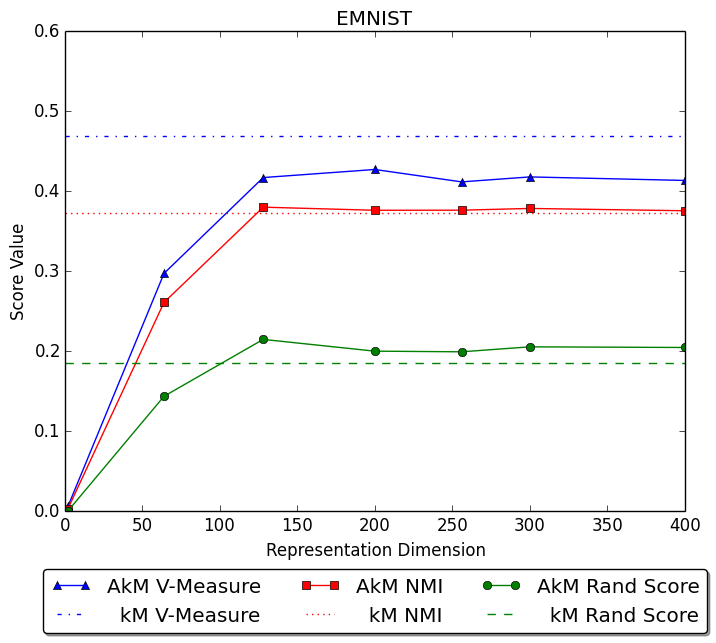
\includegraphics[width=\textwidth]{figs/emnist_graph.png}
	\end{minipage}
	\caption{Effect of representation dimension on performance. Solid lines show score values from the clusterings generated by autoencoded $k$-means (AkM). Horizontal dashed lines show score values of clusterings produced by gradient $k$-means (kM) without any autoencoder.}
	\label{fig:dims}
\end{figure}

\subsection{Effect of Noisy Data}
To evaluate the capacity  of my model to denoise data, I artificially added noise to the images. I applied a technique known as Gaussian whitening. For each pixel, a value was drawn from a zero mean Gaussian distribution with variance $\sigma^2$. This value was added to the pixel's value and then clipped so it falls in a valid range for the image (0-255). Increasing the variance results in nosier images. Figure \ref{fig:noisy} shows examples of such images. For values of $\sigma^2$ from 0 to 100, I generated a noisy dataset and trained autoencoded $k$-means to denoise this data. The best performing dimension size (256 for MNIST and 128 for EMNIST) from the previous experiments were used. Therefore autoencoded $k$-means is in fact simultaneously reducing the dimensionality of the data and denoising it. Figure \ref{fig:noise} shows that results of these experiments.

We first discuss the performance of $k$-means on noisy data. From my experiments we see that it performs poorly once the variance of the noise is $\geq 70$.  Both datasets are fairly robust to noise until that point, after which the performance sharply drops off.  In fact, we actually see a small increase in performance for small variance noise, suggesting that the noise may be introducing a minor regularization effect. Performance on the MNIST dataset especially suffers from the addition of noise, with a drop to 0 on all metrics in the worst case, meaning that $k$-means is essentially producing random clusters in that scenario.

We see that the addition of a denoising autoencoder significantly improves the clustering performance on noisy data. My experiments show that increasing the variance of the noise distribution still hurts performance, however, the decline is much less intense. We see that for noisy data with variance $\geq 70$, the performance is significantly improved. In fact, on the EMNIST dataset the performance is nearly decoupled from the amount of noise, suggesting that the autoencoder is able to completely learn the noise distribution. 

\begin{figure}
	\centering
	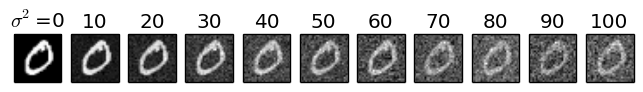
\includegraphics[width=\textwidth]{figs/noisy_row.png}
	\caption{Example of noisy images. As the variance ($\sigma^2$) of the noise distribution increases, the images are considerably more corrupted.}
	\label{fig:noisy}
\end{figure}

\begin{figure}
	\centering
	\begin{minipage}[b]{0.45\textwidth}
		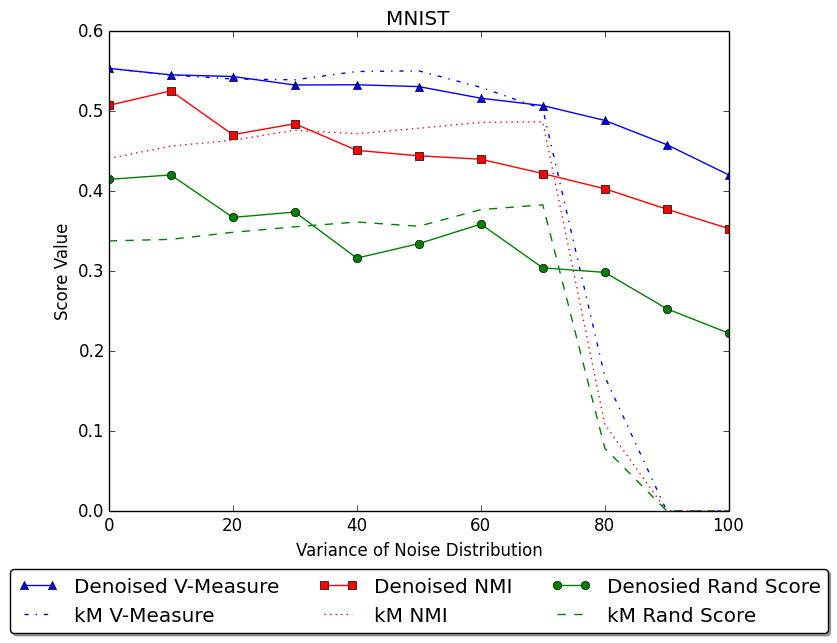
\includegraphics[width=\textwidth]{figs/mnist_noise.png}
	\end{minipage}
	\hfill
	\begin{minipage}[b]{0.45\textwidth}
		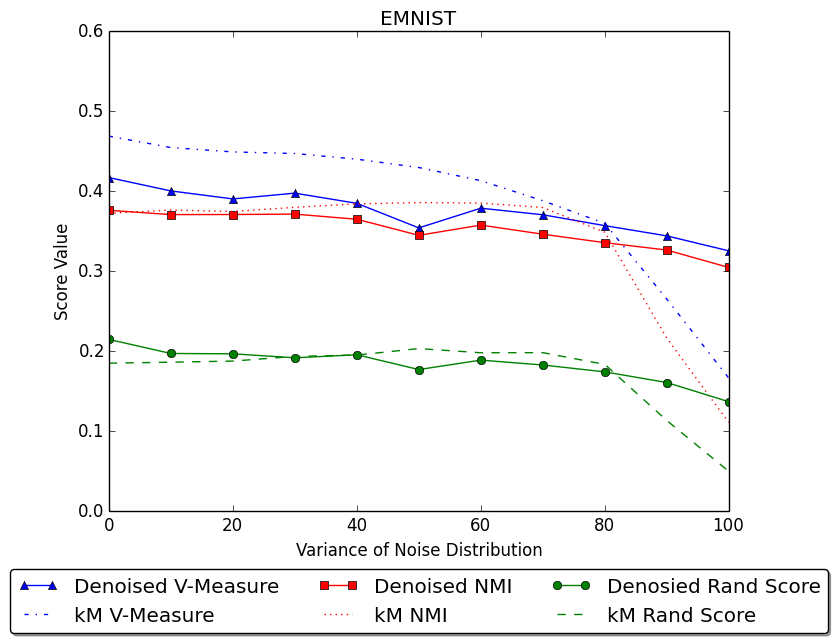
\includegraphics[width=\textwidth]{figs/emnist_noise.png}
	\end{minipage}
	\caption{Effect of noisy data on performance. Solid lines show score values from the clusterings generated by autoencoded $k$-means (with denoising) on noisy data. Dashed lines show score values of clusterings produced by gradient $k$-means (kM) without any autoencoder on the same noisy data.}
	\label{fig:noise}
\end{figure}


\section{Future Work}
The results presented here lay a reasonable groundwork for future work. The most straightforward thing to try next would be to test my model's performance on other datasets. In fact, I originally had planned to test on the CIFAR-10 color image dataset \cite{cifar}, but I discovered that the state-of-art method used 4000 clusters, which was outside of my computational budget. Additionally, it would be interesting to test my model on non-image datasets, such as textual data.

Another area to pursue would be to experiment with the autoencoder architecture. The results presented here use a very basic autoencoder, but significantly more advanced models exist. The most straightforward change would be to implement  a deep autoencoder which has many more hidden layers. Additionally, there are has been some work in using deconvolution operations which could be especially useful for the image datasets used here. In any case, it seems likely that a more sophisticated architecture could produce better lower dimensional representations, leading to better cluster performance.

\section{Conclusion}
In closing, $k$-means can perform poorly on datasets with many features or in the presence of noise. I designed and implemented autoencoded $k$-means, a neural architecture where jointly learns an autoencoder and optimizes the $k$-means objective. We see that on two image datasets, this new model performs better than $k$-means by clustering the data in a lower dimensional space. Furthermore, autoencoded $k$-means can successfully learn the noise distribution of noisy data leading to a denoising effect. This results in significantly improved performance in the presence of noise. 

\clearpage
\bibliography{sources.bib}
\bibliographystyle{ieeetr}

\iffalse
\section{Submission of papers to NIPS 2014}

NIPS requires electronic submissions.  The electronic submission site is  
\begin{center}
   \url{http://papers.nips.cc}
\end{center}

Please read carefully the
instructions below, and follow them faithfully.
\subsection{Style}

Papers to be submitted to NIPS 2014 must be prepared according to the
instructions presented here. Papers may be only up to eight pages long,
including figures. Since 2009 an additional ninth page \textit{containing only
cited references} is allowed. Papers that exceed nine pages will not be
reviewed, or in any other way considered for presentation at the conference.
%This is a strict upper bound. 

Please note that this year we have introduced automatic line number generation
into the style file (for \LaTeXe and Word versions). This is to help reviewers
refer to specific lines of the paper when they make their comments. Please do
NOT refer to these line numbers in your paper as they will be removed from the
style file for the final version of accepted papers.

The margins in 2014 are the same as since 2007, which allow for $\approx 15\%$
more words in the paper compared to earlier years. We are also again using 
double-blind reviewing. Both of these require the use of new style files.

Authors are required to use the NIPS \LaTeX{} style files obtainable at the
NIPS website as indicated below. Please make sure you use the current files and
not previous versions. Tweaking the style files may be grounds for rejection.

%% \subsection{Double-blind reviewing}

%% This year we are doing double-blind reviewing: the reviewers will not know 
%% who the authors of the paper are. For submission, the NIPS style file will 
%% automatically anonymize the author list at the beginning of the paper.

%% Please write your paper in such a way to preserve anonymity. Refer to
%% previous work by the author(s) in the third person, rather than first
%% person. Do not provide Web links to supporting material at an identifiable
%% web site.

%%\subsection{Electronic submission}
%%
%% \textbf{THE SUBMISSION DEADLINE IS June 6, 2014. SUBMISSIONS MUST BE LOGGED BY
%% 23:00, June 6, 2014, UNIVERSAL TIME}

%% You must enter your submission in the electronic submission form available at
%% the NIPS website listed above. You will be asked to enter paper title, name of
%% all authors, keyword(s), and data about the contact
%% author (name, full address, telephone, fax, and email). You will need to
%% upload an electronic (postscript or pdf) version of your paper.

%% You can upload more than one version of your paper, until the
%% submission deadline. We strongly recommended uploading your paper in
%% advance of the deadline, so you can avoid last-minute server congestion.
%%
%% Note that your submission is only valid if you get an e-mail
%% confirmation from the server. If you do not get such an e-mail, please
%% try uploading again. 


\subsection{Retrieval of style files}

The style files for NIPS and other conference information are available on the World Wide Web at
\begin{center}
   \url{http://www.nips.cc/}
\end{center}
The file \verb+nips2014.pdf+ contains these 
instructions and illustrates the
various formatting requirements your NIPS paper must satisfy. \LaTeX{}
users can choose between two style files:
\verb+nips11submit_09.sty+ (to be used with \LaTeX{} version 2.09) and
\verb+nips11submit_e.sty+ (to be used with \LaTeX{}2e). The file
\verb+nips2014.tex+ may be used as a ``shell'' for writing your paper. All you
have to do is replace the author, title, abstract, and text of the paper with
your own. The file
\verb+nips2014.rtf+ is provided as a shell for MS Word users.

The formatting instructions contained in these style files are summarized in
sections \ref{gen_inst}, \ref{headings}, and \ref{others} below.

%% \subsection{Keywords for paper submission}
%% Your NIPS paper can be submitted with any of the following keywords (more than one keyword is possible for each paper):

%% \begin{verbatim}
%% Bioinformatics
%% Biological Vision
%% Brain Imaging and Brain Computer Interfacing
%% Clustering
%% Cognitive Science
%% Control and Reinforcement Learning
%% Dimensionality Reduction and Manifolds
%% Feature Selection
%% Gaussian Processes
%% Graphical Models
%% Hardware Technologies
%% Kernels
%% Learning Theory
%% Machine Vision
%% Margins and Boosting
%% Neural Networks
%% Neuroscience
%% Other Algorithms and Architectures
%% Other Applications
%% Semi-supervised Learning
%% Speech and Signal Processing
%% Text and Language Applications

%% \end{verbatim}

\section{General formatting instructions}
\label{gen_inst}

The text must be confined within a rectangle 5.5~inches (33~picas) wide and
9~inches (54~picas) long. The left margin is 1.5~inch (9~picas).
Use 10~point type with a vertical spacing of 11~points. Times New Roman is the
preferred typeface throughout. Paragraphs are separated by 1/2~line space,
with no indentation.

Paper title is 17~point, initial caps/lower case, bold, centered between
2~horizontal rules. Top rule is 4~points thick and bottom rule is 1~point
thick. Allow 1/4~inch space above and below title to rules. All pages should
start at 1~inch (6~picas) from the top of the page.

%The version of the paper submitted for review should have ``Anonymous Author(s)'' as the author of the paper.

For the final version, authors' names are
set in boldface, and each name is centered above the corresponding
address. The lead author's name is to be listed first (left-most), and
the co-authors' names (if different address) are set to follow. If
there is only one co-author, list both author and co-author side by side.

Please pay special attention to the instructions in section \ref{others}
regarding figures, tables, acknowledgments, and references.

\section{Headings: first level}
\label{headings}

First level headings are lower case (except for first word and proper nouns),
flush left, bold and in point size 12. One line space before the first level
heading and 1/2~line space after the first level heading.

\subsection{Headings: second level}

Second level headings are lower case (except for first word and proper nouns),
flush left, bold and in point size 10. One line space before the second level
heading and 1/2~line space after the second level heading.

\subsubsection{Headings: third level}

Third level headings are lower case (except for first word and proper nouns),
flush left, bold and in point size 10. One line space before the third level
heading and 1/2~line space after the third level heading.

\section{Citations, figures, tables, references}
\label{others}

These instructions apply to everyone, regardless of the formatter being used.

\subsection{Citations within the text}

Citations within the text should be numbered consecutively. The corresponding
number is to appear enclosed in square brackets, such as [1] or [2]-[5]. The
corresponding references are to be listed in the same order at the end of the
paper, in the \textbf{References} section. (Note: the standard
\textsc{Bib\TeX} style \texttt{unsrt} produces this.) As to the format of the
references themselves, any style is acceptable as long as it is used
consistently.

As submission is double blind, refer to your own published work in the 
third person. That is, use ``In the previous work of Jones et al.\ [4]'',
not ``In our previous work [4]''. If you cite your other papers that
are not widely available (e.g.\ a journal paper under review), use
anonymous author names in the citation, e.g.\ an author of the
form ``A.\ Anonymous''. 


\subsection{Footnotes}

Indicate footnotes with a number\footnote{Sample of the first footnote} in the
text. Place the footnotes at the bottom of the page on which they appear.
Precede the footnote with a horizontal rule of 2~inches
(12~picas).\footnote{Sample of the second footnote}

\subsection{Figures}

All artwork must be neat, clean, and legible. Lines should be dark
enough for purposes of reproduction; art work should not be
hand-drawn. The figure number and caption always appear after the
figure. Place one line space before the figure caption, and one line
space after the figure. The figure caption is lower case (except for
first word and proper nouns); figures are numbered consecutively.

Make sure the figure caption does not get separated from the figure.
Leave sufficient space to avoid splitting the figure and figure caption.

You may use color figures. 
However, it is best for the
figure captions and the paper body to make sense if the paper is printed
either in black/white or in color.
\begin{figure}[h]
\begin{center}
%\framebox[4.0in]{$\;$}
\fbox{\rule[-.5cm]{0cm}{4cm} \rule[-.5cm]{4cm}{0cm}}
\end{center}
\caption{Sample figure caption.}
\end{figure}

\subsection{Tables}

All tables must be centered, neat, clean and legible. Do not use hand-drawn
tables. The table number and title always appear before the table. See
Table~\ref{sample-table}.

Place one line space before the table title, one line space after the table
title, and one line space after the table. The table title must be lower case
(except for first word and proper nouns); tables are numbered consecutively.

\begin{table}[t]
\caption{Sample table title}
\label{sample-table}
\begin{center}
\begin{tabular}{ll}
\multicolumn{1}{c}{\bf PART}  &\multicolumn{1}{c}{\bf DESCRIPTION}
\\ \hline \\
Dendrite         &Input terminal \\
Axon             &Output terminal \\
Soma             &Cell body (contains cell nucleus) \\
\end{tabular}
\end{center}
\end{table}

\section{Final instructions}
Do not change any aspects of the formatting parameters in the style files.
In particular, do not modify the width or length of the rectangle the text
should fit into, and do not change font sizes (except perhaps in the
\textbf{References} section; see below). Please note that pages should be
numbered.

\section{Preparing PostScript or PDF files}

Please prepare PostScript or PDF files with paper size ``US Letter'', and
not, for example, ``A4''. The -t
letter option on dvips will produce US Letter files.

Fonts were the main cause of problems in the past years. Your PDF file must
only contain Type 1 or Embedded TrueType fonts. Here are a few instructions
to achieve this.

\begin{itemize}

\item You can check which fonts a PDF files uses.  In Acrobat Reader,
select the menu Files$>$Document Properties$>$Fonts and select Show All Fonts. You can
also use the program \verb+pdffonts+ which comes with \verb+xpdf+ and is
available out-of-the-box on most Linux machines.

\item The IEEE has recommendations for generating PDF files whose fonts
are also acceptable for NIPS. Please see
\url{http://www.emfield.org/icuwb2010/downloads/IEEE-PDF-SpecV32.pdf}

\item LaTeX users:

\begin{itemize}

\item Consider directly generating PDF files using \verb+pdflatex+
(especially if you are a MiKTeX user). 
PDF figures must be substituted for EPS figures, however.

\item Otherwise, please generate your PostScript and PDF files with the following commands:
\begin{verbatim} 
dvips mypaper.dvi -t letter -Ppdf -G0 -o mypaper.ps
ps2pdf mypaper.ps mypaper.pdf
\end{verbatim}

Check that the PDF files only contains Type 1 fonts. 
%For the final version, please send us both the Postscript file and
%the PDF file. 

\item xfig "patterned" shapes are implemented with 
bitmap fonts.  Use "solid" shapes instead. 
\item The \verb+\bbold+ package almost always uses bitmap
fonts.  You can try the equivalent AMS Fonts with command
\begin{verbatim}
\usepackage[psamsfonts]{amssymb}
\end{verbatim}
 or use the following workaround for reals, natural and complex: 
\begin{verbatim}
\newcommand{\RR}{I\!\!R} %real numbers
\newcommand{\Nat}{I\!\!N} %natural numbers 
\newcommand{\CC}{I\!\!\!\!C} %complex numbers
\end{verbatim}

\item Sometimes the problematic fonts are used in figures
included in LaTeX files. The ghostscript program \verb+eps2eps+ is the simplest
way to clean such figures. For black and white figures, slightly better
results can be achieved with program \verb+potrace+.
\end{itemize}
\item MSWord and Windows users (via PDF file):
\begin{itemize}
\item Install the Microsoft Save as PDF Office 2007 Add-in from
\url{http://www.microsoft.com/downloads/details.aspx?displaylang=en\&familyid=4d951911-3e7e-4ae6-b059-a2e79ed87041}
\item Select ``Save or Publish to PDF'' from the Office or File menu
\end{itemize}
\item MSWord and Mac OS X users (via PDF file):
\begin{itemize}
\item From the print menu, click the PDF drop-down box, and select ``Save
as PDF...''
\end{itemize}
\item MSWord and Windows users (via PS file):
\begin{itemize}
\item To create a new printer
on your computer, install the AdobePS printer driver and the Adobe Distiller PPD file from
\url{http://www.adobe.com/support/downloads/detail.jsp?ftpID=204} {\it Note:} You must reboot your PC after installing the
AdobePS driver for it to take effect.
\item To produce the ps file, select ``Print'' from the MS app, choose
the installed AdobePS printer, click on ``Properties'', click on ``Advanced.''
\item Set ``TrueType Font'' to be ``Download as Softfont''
\item Open the ``PostScript Options'' folder
\item Select ``PostScript Output Option'' to be ``Optimize for Portability''
\item Select ``TrueType Font Download Option'' to be ``Outline''
\item Select ``Send PostScript Error Handler'' to be ``No''
\item Click ``OK'' three times, print your file.
\item Now, use Adobe Acrobat Distiller or ps2pdf to create a PDF file from
the PS file. In Acrobat, check the option ``Embed all fonts'' if
applicable.
\end{itemize}

\end{itemize}
If your file contains Type 3 fonts or non embedded TrueType fonts, we will
ask you to fix it. 

\subsection{Margins in LaTeX}
 
Most of the margin problems come from figures positioned by hand using
\verb+\special+ or other commands. We suggest using the command
\verb+\includegraphics+
from the graphicx package. Always specify the figure width as a multiple of
the line width as in the example below using .eps graphics
\begin{verbatim}
   \usepackage[dvips]{graphicx} ... 
   \includegraphics[width=0.8\linewidth]{myfile.eps} 
\end{verbatim}
or % Apr 2009 addition
\begin{verbatim}
   \usepackage[pdftex]{graphicx} ... 
   \includegraphics[width=0.8\linewidth]{myfile.pdf} 
\end{verbatim}
for .pdf graphics. 
See section 4.4 in the graphics bundle documentation (\url{http://www.ctan.org/tex-archive/macros/latex/required/graphics/grfguide.ps}) 
 
A number of width problems arise when LaTeX cannot properly hyphenate a
line. Please give LaTeX hyphenation hints using the \verb+\-+ command.


\subsubsection*{Acknowledgments}

Use unnumbered third level headings for the acknowledgments. All
acknowledgments go at the end of the paper. Do not include 
acknowledgments in the anonymized submission, only in the 
final paper. 

\subsubsection*{References}

References follow the acknowledgments. Use unnumbered third level heading for
the references. Any choice of citation style is acceptable as long as you are
consistent. It is permissible to reduce the font size to `small' (9-point) 
when listing the references. {\bf Remember that this year you can use
a ninth page as long as it contains \emph{only} cited references.}

\small{
[1] Alexander, J.A. \& Mozer, M.C. (1995) Template-based algorithms
for connectionist rule extraction. In G. Tesauro, D. S. Touretzky
and T.K. Leen (eds.), {\it Advances in Neural Information Processing
Systems 7}, pp. 609-616. Cambridge, MA: MIT Press.

[2] Bower, J.M. \& Beeman, D. (1995) {\it The Book of GENESIS: Exploring
Realistic Neural Models with the GEneral NEural SImulation System.}
New York: TELOS/Springer-Verlag.

[3] Hasselmo, M.E., Schnell, E. \& Barkai, E. (1995) Dynamics of learning
and recall at excitatory recurrent synapses and cholinergic modulation
in rat hippocampal region CA3. {\it Journal of Neuroscience}
{\bf 15}(7):5249-5262.
}

\fi

\end{document}